\documentclass[11pt]{article}
\usepackage[margin=1in]{geometry}
\usepackage{fancyhdr}
\usepackage{enumitem}
\usepackage{parskip}
\usepackage{xcolor}
\usepackage{graphicx}
\usepackage{amssymb}
\usepackage{amsmath}
\usepackage{array}
\usepackage[margin=1in]{geometry}

% Personal notes: \comment{Write your thoughts here.}
% Notes appear in grey in the compiled document; blank lines are supported.
\definecolor{commentgray}{gray}{0.5}
\newcommand{\comment}[1]{{\color{commentgray}#1}}

\pagestyle{fancy}
\fancyhf{}
\fancyhead[C]{\textbf{CEG2136}}
\fancyfoot[C]{\thepage}

\newcounter{chapterNumber}
\setcounter{chapterNumber}{1}
\newcounter{headerOneCount}
\newcounter{headerTwoCount}[headerOneCount]
\setcounter{headerOneCount}{-1}
\renewcommand{\theheaderOneCount}{\arabic{headerOneCount}}
\renewcommand{\theheaderTwoCount}{\arabic{headerTwoCount}}

\newcommand{\Title}[1]{%
  \begin{center}
    \fontsize{24}{28}\selectfont\textbf{#1}
  \end{center}
  \vspace{1em}
}

\newcommand{\HeaderOne}[1]{%
  \refstepcounter{headerOneCount}%
  \setcounter{headerTwoCount}{-1}%
  \vspace{0.75em}
  \noindent\fontsize{18}{22}\selectfont\textbf{\arabic{chapterNumber}.\theheaderOneCount\ #1}\par
  \vspace{0.5em}
}

\newcommand{\HeaderTwo}[1]{%
  \refstepcounter{headerTwoCount}%
  \vspace{0.5em}
  \noindent\fontsize{16}{20}\selectfont\textbf{\arabic{chapterNumber}.\theheaderOneCount.\theheaderTwoCount\ #1}\par
  \vspace{0.4em}
}

\newcommand{\BodyText}[1]{%
  \fontsize{12}{15}\selectfont #1\par
}




\newenvironment{NumberedList}{%
  \begin{enumerate}[leftmargin=2em, itemsep=0.35em, topsep=0.35em]
}{%
  \end{enumerate}
}

\newenvironment{DottedList}{%
  \begin{itemize}[leftmargin=2em, itemsep=0.35em, topsep=0.35em, label=\textbullet]
}{%
  \end{itemize}
}

\begin{document}

\title{Computer Organization}

\section{Instruction List}

\textit{The instructions list is the list of \textbf{physically implemented} instructions in the computer}

\subsection{Instruction Codes}

A compiler reads code and converts it to instructions codes. 
\begin{itemize}
  \item Instruction code are groups of bits (binary code) that instruct the computer to perform a sequence of micro-operations.
  \begin{itemize}
    \item These instruction codes can be shortened to be \textbf{human-readable}, which is how we end up with the \textbf{Basic Computer Instruction List}.
  \end{itemize}
  \item Instruction codes are divided into two parts:
  \begin{itemize}
    \item Operation code (opcode) and Address code
    \begin{itemize}
      \item Opcode defines operation to be performed
      \item Address code refers to the operands in some way (expanded upon in addressing modes)
    \end{itemize} 
  \end{itemize}
  \item \textit{But Nathan! How does the computer read these instruction codes?}
  \begin{NumberedList}
  \item Control Unit (CU) reads the instruction code from the instruction register 
  \item CU outputs control signals that initiate the necessary sequence of micro-operations on the specified operands. 
  \end{NumberedList}
  \item This process is called \textbf{fetch-decode cycle} OR the \textbf{Instruction Cycle} 
\end{itemize}

\subsubsection{Instruction Codes: Bit by Bit}
\textit{Instruction codes must specify not only the operation, but also the registers or memory cells of the operands, and the result data locations}

\begin{itemize}
  \item $IR_{15}$, denotes the type of memory addressing: CPU Registers or Memory Cells
  \item $IR_{14-12}$, regard the actual operation instructions
  \item $IR_{11-0}$, are for the operand data. 
\end{itemize}

\section{The Control Unit}
Consists of:
\begin{itemize}
  \item Instruction Decoder: A decoder dedicated for $IR_{14-12}$ and decoding what operations we want
  \item State Register: A sequence counter and a decoder. 
  \begin{itemize}
    \item The state register counts each sequential step of completing an operation. 
    \item Outputs timing signals, which are signals that show what step an operation is at.
  \end{itemize}
  \item Control Logic Gates: Takes \textbf{timing signals} and \textbf{Instruction decoder signals }and outputs \textbf{Control Signals}
\end{itemize}
For any instruction code, the timing signals and instruction decode signals will be different. The control signals are send to buses, MUXes and the AC unit. 

\section{Instruction Cycle}
\textit{The cycle where a computer reads an instruction code, executes and ends.}
\subsection{Fetch and Decode}
\textit{The first 4 timing signals (State Register $T_0$ - $T_3$) are specifically used for fetching and decoding the data in the instruction register}
\begin{NumberedList}
  \item $T_0$: AR $\leftarrow$ PC 
  \item $T_1$: IR $\leftarrow$ M[AR], PC $\leftarrow$ PC + 1
  \item $T_2$: $D_0$,...,$D_7$ $\leftarrow$ Decode IR(12-14), AR $\leftarrow$ IR(0-11), I $\leftarrow$ IR(15)
  \item $T_3$: Varies based on the type of operation.
\end{NumberedList}
\textbf{After fetch and decode, the operation and operands are known, so we begin the operation.}

\subsection{Register Reference Instructions}
\textit{Post fetch and decode, $T_3$ and onwards. Directly accessing CPU registers (AC). $D_7$ = 1, I = 0.\\}
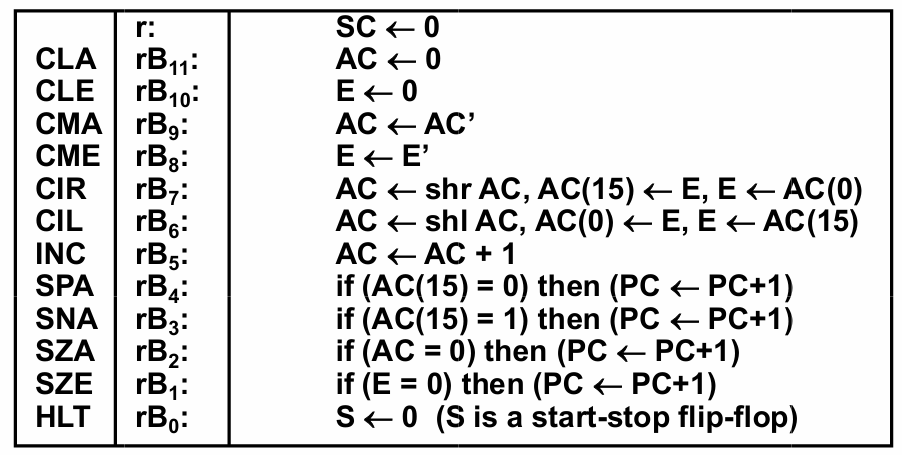
\includegraphics[width=1\textwidth]{RegisterReferenceInstructions.png}

\subsection{Memory Reference Instructions}
\textit{Post fetch and decode, $T_3$ and onwards. $D_i$ = 1, I = ${0..6}$}
\begin{itemize}
  \item At $T_2$ we obtained the Decoder signals, each of these decoder signals denotes one operation. 
  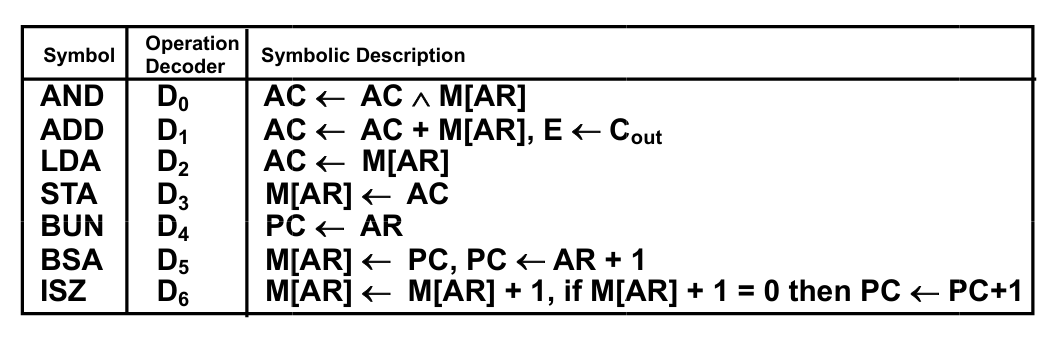
\includegraphics[width=1\textwidth]{MemoryReferenceInstructions.png}
  \item Realistically, each operation requires more than one timing signal (pulses) and are not just one notation. 

  \item AND to AC
  \begin{itemize}
    \item RTL Notation: AC $\leftarrow$ AC $\land$ M[AR] 
    \begin{itemize}
      \item $D_0$$T_4$: DR $\leftarrow$ M[AR] Read operand 
      \item $D_0$$T_5$: AC $\leftarrow$ AC $\land$ DR, SC $\leftarrow$ 0 AND with AC, END program (SC $\leftarrow$ 0)
    \end{itemize}
  \end{itemize}

  \item ADD to AC
  \begin{itemize}
    \item RTL Notation: AC $\leftarrow$ AC + M[AR], E $\leftarrow$ $C_{out}$
    \begin{itemize}
      \item $D_1$$T_4$: DR $\leftarrow$ M[AR] Read operand 
      \item $D_1$$T_5$: AC $\leftarrow$ AC + DR, SC $\leftarrow$ 0, E $\leftarrow$ $C_{out}$
      \begin{itemize}
        \item E is the extend one-bit that is dedicated specifically to AC.
        \item Can also be used for signed and unsigned arithmetic. This includes shifting. 
      \end{itemize}
    \end{itemize}
  \end{itemize}
      
  \item LDA: Load to AC
  \begin{itemize}
    \item RTL Notation: AC $\leftarrow$ M[AR]
    \begin{itemize}
      \item $D_2$$T_4$: DR $\leftarrow$ M[AR] Read operand 
      \item $D_2$$T_5$: AC $\leftarrow$ DR, SC $\leftarrow$ 0 Store/Load DR in AC
    \end{itemize}
  \end{itemize}

  \item STA: Store AC
  \begin{itemize}
    \item RTL Notation: M[AR] $\leftarrow$ AC
    \begin{itemize}
      \item $D_3$$T_4$: M[AR] $\leftarrow$ AC, SC $\leftarrow$ 0
    \end{itemize}
  \end{itemize}

  \item BUN: Branch Unconditionally
  \begin{itemize}
    \item $D_3$$T_4$: PC $\leftarrow$ AR, SC $\leftarrow$ 0
  \end{itemize}

  \item BSA: Branch and Save Return Address
  \begin{itemize}
    \item RTL Notation: M[AR] $\leftarrow$ PC, PC $\leftarrow$ AR + 1
    \begin{itemize}
      \item $D_5$$T_4$: M[AR] $\leftarrow$ PC, AC $\leftarrow$ AR + 1
      \item $D_5$$T_5$: PC $\leftarrow$ AR, SC $\leftarrow$ 0
    \end{itemize}
  \end{itemize}

  \item ISZ: Increment and Skip-if-Zero
  \begin{itemize}
    \item $D_6$$T_4$: DR $\leftarrow$ M[AR]
    \item $D_6$$T_5$: DR $\leftarrow$ DR + 1
    \item $D_6$$T_6$: M[AR] $\leftarrow$ DR, if (DR = 0) then (PC $\leftarrow$ + 1), SC $\leftarrow$ 0
  \end{itemize}

\end{itemize}

\subsection{Subroutines}
\textit{A subroutine is a task that pauses the main task (program) until completion.}
\begin{itemize}
  \item All subroutines use BSA: Branch and Save Return Address.
  \item Once subroutine is completed BUN (Branch Unconditionally) is used to return to the saved return address.=
\end{itemize}

\subsubsection{Types of Subroutines}
Generally, there are two types, Interrupts and Execution:
\begin{itemize}
  \item Execution can be broken down further into:
  \begin{itemize}
    \item Leaf Subroutine: Does not call any other subroutine. It executes its instructions and returns directly to the caller.
    \item Nested Subroutine: Calls another subroutine. Multiple return addresses must be preserved.
    \item Recursive Subroutine: Calls itself until a base case is satisfied. Each invocation generally requires its own stack frame.
  \end{itemize}
  \item Interrupt service routine (ISR): Triggered by an interrupt rather than an ordinary subroutine call. It preserves the necessary processor state before resuming execution.
\end{itemize}

\subsubsection{Input-Output Process}
\textit{Instructions and data in memory must come from an input device, computed results must be outputted to some output device.}
\begin{itemize}
  \item To communicate with an input device, we use the input register INPR.
  \item To output information, it is stored in the output register OUTR.
  \item FGI (Flag Input) and FGO (Flag Output) are 1-bit flip flops that tracks new information 
  \begin{itemize}
    \item FGI is set to 1 when a new information is available in the input device and is cleared to 0 when the information is accepted by the computer.
    \item If FGO is set to 1, then this means that the computer can send out the information from AC. If it is 0, then the output device is busy and the computer has to wait.
  \end{itemize}
  \item The inputting process
  \begin{itemize}
    \item FGI = 0
    \item 8-bit alphanumeric code is shifted into INPR (keyboard input) and FGI = 1
    \item If FGI = 1: AC $\leftarrow$ INPR, FGI $\leftarrow$ 0
  \end{itemize}
  \item The outputting process
  \begin{itemize}
    \item FGO = 1
    \item IF FGO = 1: OUTR $\leftarrow$ AC, FGO $\leftarrow$ 0
    \item OUTR is printed
    \item When operation is completed FGO = 1.
  \end{itemize}
\end{itemize}

\subsection{Input-Output Instructions}
\textit{Post fetch and decode, $T_3$ and onwards. Used for transferring data to and from AC, checking flag bits and controlling the interrupt subroutines.\\}
$D_{7}IT_{3}$ = p (Instruct Decode 7, Indirect Mode, and at $T_3$)\\ 
$IR_i$ = $B_i$, i = 6,..., 11 \\
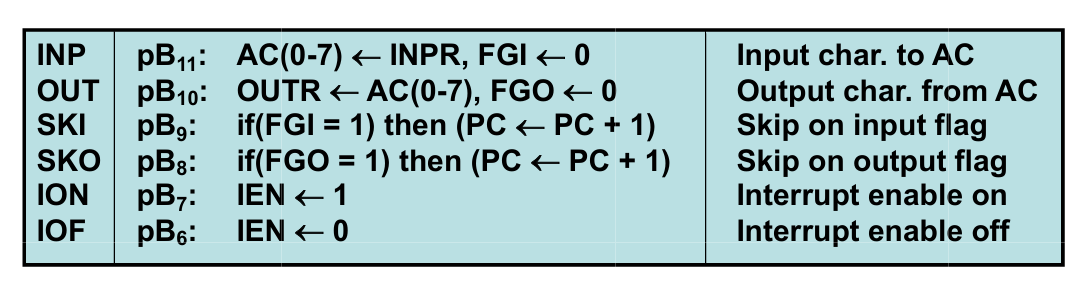
\includegraphics[width=1\textwidth]{InputOutputInstructions.png}

\subsection{Program Interrupt}
\textit{Problem: CPU repeatedly checks (waste of time) the status of an external device using flag bits. If Flag = 1, Transfer data. This is sometimes called polling (checking and transferring)}
\textbf{Solution: Program Interrupt. External device informs the computer when it is ready for transfer, this utilizes the interrupt facility. (Internal Asynchronous CPU Timing)}
\newpage
\begin{minipage}{0.28\textwidth}
  \centering
  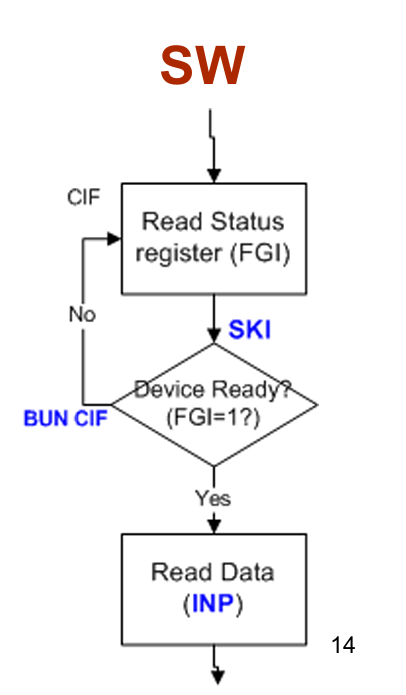
\includegraphics[width=\linewidth]{SoftwarePolling.png}
\end{minipage}\hfill
\begin{minipage}{0.58\textwidth}
  \centering
  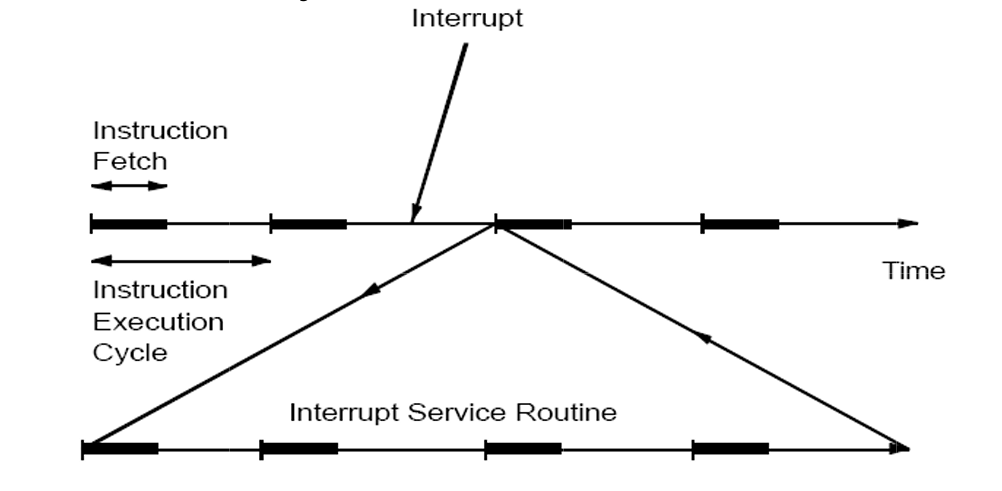
\includegraphics[width=\linewidth]{InternalAsyncCPUTiming.png}
\end{minipage}
\begin{center}
  \item Figure: Software Polling vs Internal Asynchronous CPU Timing\\
\end{center}

\begin{itemize}
  \item When a flag is set, a program interrupt occurs. Input-Output transfer is taken care of, then computer returns to program.
  \item The interrupt facility is controlled by a flip-flop: IEN.
  \item IEN denotes whether or not an interrupt can take place or not. It is set and cleared with two instructions
  \begin{itemize}
    \item IOF: IEN $\leftarrow$ 0 (no interrupts)
    \item ION: IEN $\leftarrow$ 1 (yes interrupts)
  \end{itemize}
  \item Interrupt Cycle flip-flop: R. 
  \item R controls when to go through an interrupt cycle.
\end{itemize}

\end{document}
